% !TEX TS-program = pdflatex
% !TEX encoding = UTF-8 Unicode
\documentclass{article} % use larger type; default would be 10pt

\usepackage[utf8]{inputenc} % set input encoding (not needed with XeLaTeX)

%%% PAGE DIMENSIONS
\usepackage{geometry} % to change the page dimensions
\geometry{a4paper} % or letterpaper (US) or a5paper or....
\geometry{margin=1in} % for example, change the margins to 2 inches all round
% \geometry{landscape} % set up the page for landscape
%   read geometry.pdf for detailed page layout information

\usepackage{graphicx} % support the \includegraphics command and options

 \usepackage[parfill]{parskip} % Activate to begin paragraphs with an empty line rather than an indent

%%% PACKAGES
\usepackage{booktabs} % for much better looking tables
\usepackage{array} % for better arrays (eg matrices) in maths
\usepackage{paralist} % very flexible & customisable lists (eg. enumerate/itemize, etc.)
\usepackage{verbatim} % adds environment for commenting out blocks of text & for better verbatim
\usepackage{subfig} % make it possible to include more than one captioned figure/table in a single float

\usepackage[usenames,dvipsnames]{color}
\usepackage{textcomp}
\usepackage{listings}
\lstset{ 
language=Python,                % choose the language of the code
basicstyle=\scriptsize,       % the size of the fonts that are used for the code
identifierstyle=\ttfamily,
numbers=left,                   % where to put the line-numbers
numberstyle=\ttfamily,      % the size of the fonts that are used for the line-numbers
stepnumber=1,                   % the step between two line-numbers. If it is 1 each line will be numbered
numbersep=2pt,                  % how far the line-numbers are from the code
backgroundcolor=\color[rgb]{0.95,.95,.95},  % choose the background color. You must add \usepackage{color}
showspaces=false,               % show spaces adding particular underscores
showstringspaces=false,         % underline spaces within strings
showtabs=false,                 % show tabs within strings adding particular underscores
%frame=single,   		% adds a frame around the code
tabsize=2,  		% sets default tabsize to 2 spaces
captionpos=b,   		% sets the caption-position to bottom
breaklines=true,    	% sets automatic line breaking
breakatwhitespace=false,    % sets if automatic breaks should only happen at whitespace
escapeinside={\%*}{*},          % if you want to add a comment within your code
upquote=true,
keywordstyle=\color{blue}\ttfamily,
commentstyle=\ttfamily\color{ForestGreen},
upquote=true,
morekeywords={True,False,None,self,cls},
otherkeywords = {1,2,3,4,5,6,7,8,9,0,+,=,-,/},
stringstyle=\color{red}\ttfamily,
keywordsprefix = @
}

\newenvironment{inset}
{
\begin{center}
\begin{minipage}{0.85\textwidth}
}
{
\end{minipage}
\end{center}
}

\makeatletter
\lst@AddToHook{TextStyle}{\let\lst@basicstyle\ttfamily\normalsize\fontfamily{pcr}\selectfont}
\makeatother

%shorthand for inline listings, also prevents linebreaks in code
\newcommand{\il}[1]{\mbox{\lstinline{#1}}}

\newcommand{\lstslice}[3]{
\begin{inset}
\lstinputlisting[nolol=true, linerange={#1-#2}, firstnumber=#1]{#3}
\end{inset}
}
\usepackage{xargs}
\newcommandx{\lstdump}[3][1=1,2=No Caption]{
\begin{inset}
\newcommand{\storelstname}{\lstlistingname}
\newcommand{\storelstlisting}{\thelstlisting}
%\renewcommand{\lstlistingname}{#1}
%\renewcommand{\thelstlisting}{}
\lstinputlisting[name=#1, caption={#1 -- #2}]{#3}
%\renewcommand{\lstlistingname}{\storelstname}
%\renewcommand{\thelstlisting}{\storelstlisting}
\end{inset}
}

\newcounter{SessionCounter}
\setcounter{SessionCounter}{0}

\newcommand{\lstsession}[2][No Caption]{
\stepcounter{SessionCounter}
\lstdump[Session \arabic{SessionCounter}][#1]{#2}
}

%%% HEADERS & FOOTERS
\usepackage{fancyhdr} % This should be set AFTER setting up the page geometry
\pagestyle{fancy} % options: empty , plain , fancy
\renewcommand{\headrulewidth}{0pt} % customise the layout...
\lhead{QUI}\chead{}\rhead{J.H., H.S.}
\lfoot{}\cfoot{\thepage}\rfoot{}

%%% SECTION TITLE APPEARANCE
\usepackage{sectsty}
\allsectionsfont{\sffamily\mdseries\upshape} % (See the fntguide.pdf for font help)
% (This matches ConTeXt defaults)

%%% ToC (table of contents) APPEARANCE
\usepackage[nottoc,notlof,notlot]{tocbibind} % Put the bibliography in the ToC
\usepackage[titles,subfigure]{tocloft} % Alter the style of the Table of Contents
\renewcommand{\cftsecfont}{\rmfamily\mdseries\upshape}
\renewcommand{\cftsecpagefont}{\rmfamily\mdseries\upshape} % No bold!

%%% END Article customizations

%%% The "real" document content comes below...

\title{Query Universal Interface}
\author{Haak Saxberg and Jess Hester}
\date{December 9, 2011}

\begin{document}
\maketitle
\newpage

\tableofcontents
\lstlistoflistings
\listoffigures

\newpage
\section{Introduction}
The need to store persistent data is a headache for many developers. Often, they encounter this problem early on, and due to time
or budget pressure, their solution is necessarily tailored to the current realities of their applications -- with a limited view, if any, of 
their application's future, scaled-up needs.

This makes transporting an application from one storage engine to another a time-consuming and expensive affair; all too often, the
costs associated with the migration prevent the application from migrating for an extended period of time, which generally means that
users aren't getting 100\% use.

In the past, this issue was annoying but manageable, since persistent storage was frequently implemented using relational databases.
By the mid 90's, nearly all relational databases were mostly SQL-compliant. Every vendor, of course, had their own flavor of SQL which
presented the eternal threat that a critical query wouldn't run on a new database, but for the most part SQL was SQL.

However, there were issues with this approach. Relational databases are inherently constricting --- adding new entries to an already-extant 
database table is easy, but modifying a table to allow for different entry attributes requires halting all user interaction with the table while
the table is modified. For popular applications, this presents a nontrivial amount of downtime for a potentially large number of displeased 
users (see Appendix A for more discussion of the two structures).

In the modern era, companies are increasingly looking to non-relational databases as storage solutions, because they can be scaled up
much more cost-effectively and quickly -- a must in today's data-driven business world. However, non-relational databases don't yet have
a common language like SQL; one database's SELECT could very well be another's INSERT.

Enter the Query Universal Interface (QUI).

QUI attempts to ease the transition between non-relational databases, like other ORMs do for relational databases. QUI does not pretend
to implement a universal querying syntax, but rather a universal interface through which code can talk to data with minimal, if any, change.

\newpage
%%%%%%%%%%%%%%%%%%%%%%%%%%%%%%%%	SECTION 2	%%%%%%%%%%%%%%%%%%%%%%%%%%%%%%%%%%%
\section{Language Overview}
\subsection{Basic Computation}
At its heart, QUI is a translation engine. It converts class-like data into a form that is understandable to a backend's API. This form, obviously, can
vary quite a bit between databases (thus, the need for QUI in the first place) --- and the method of translation is unfortunately specific to each
backend.

An overview, however, is possible. QUI translates its own models (user-defined, of course) into what we internally refer to as an interface, which uses
the language of the backend specified by the user; this interface is what allows QUI to talk to the backend. Currently, model instance's interface is only 
created when necessary (during getting and putting), in order to reduce the memory overhead that QUI entails. 

In our tests, the performance gains garnered by storing the interface as an instance attribute are not noticeable, especially as models typically 
have fewer than 20 attributes at a time. Since interfaces are generally classes in their own right, however, they can double (or more) the size of 
the instance if they're stored; this cost can quickly add up, if the user were to \il{get}/\il{put} numerous \il{Model}s.

\subsection{Basic Data Structures}
QUI has two foundational elements: \il{Model}s and \il{Field}s. These are both abstract classes; their purpose is more to serve as interface specifications
for the rest of QUI --- any future extensions, even those written by others, are guaranteed to integrate seamlessly (as far as QUI is concerned)
as long as they honor the requirements of these two root classes. 

There are two other 'core' classes behind QUI---\il{ModelMixin} and \il{FieldMixin}, which serve similar purposes to \il{Model} and \il{Field}: interface
 requirements, which any future backend mixins need to implement in order to be considered valid. In general, \il{ModelMixin}'s subclasses are used
to add the functionality that \il{Model} requires of \emph{its} subclasses; likewise with \il{FieldMixin}'s subclasses and \il{Field}'s.

\subsection{Basic Control Structures}
Users can fine-tune their interactions with their databases in a couple of ways:
\begin{enumerate}
\item Trivially, by configuring the packaged \il{Field} subclasses (using keyword arguments defined as part of their model)
\item Defining their own \il{Field} subclasses, with custom behaviors
\item Defining their own \il{FieldMixin}s, customizing data requirements of their \il{Model}s
\item Defining their own \il{ModelMixin}s, customizing their interaction with the databases
\end{enumerate}
Apart from these, QUI's control structures are Python's control structures, since QUI is an internal DSL.

Users can configure a \il{Field} by defining an \il{Options} class inside their \il{Model} definition; currently, \il{Field}s only know how to handle the
`default' option, which sets their value at the time of their initialization. So, if we had a \il{BooleanField} named \il{is_safe}, and wanted it to default to
\il{False}, we'd define the inline class \il{Options} thus:
\begin{inset}
\begin{lstlisting}
class Options:
    is_safe = {'default':False}
\end{lstlisting}
\end{inset}
A \il{Field}'s normal validation behavior will apply to any defaults; if the default value is invalid for the field type, QUI will raise an exception when the \il{Field} is first
initialized. 
Creating custom \il{Field}s, \il{FieldMixin}s, and \il{ModelMixin}s is outside the scope of this report,
but works the same way as subclassing any other new-style Python abstract metaclass; as long as you implement the required methods, you have a ``valid"
subclass with which QUI can work. Whether or not it works the way you intend is an entirely different matter.

\subsection{Input/Output}
As input, QUI will accept a valid Python class definition. As output, QUI gives users...an altered (dare we say, improved?) class definition.
A QUI model need never use the extra methods provided by QUI; model classes can be instantiated just like any other class. Thus, declaring
a class to be a QUI model necessitates zero changes to any existing code besides the class definition.

\subsection{Error Handling}
QUI defines several custom subclasses of \il{Exception}, \il{QUIException}, so that the
user can be informed about exactly what QUI thinks has gone wrong, and where, and with what values.
QUI implements a few ``levels'' of exception, insofar as Python supports ``levels'' of program running. At the ``compilation'' level, QUI
raises \il{ImproperlyConfigured} exceptions for any settings that are not valid or missing, with appropriate error messages alongside.

Every time a \il{QUIException}, or one of its derived exceptions, is raised, QUI prints an informative error message, detailing its best
guess for what caused the exception. Along side, it prints the exception raised by the raw Python---just in case the guess is wrong.

Figure~\ref{fig:exceptionhier} describes the exceptions provided by QUI, and their relation to each other.
\begin{figure}[htb]
\centering
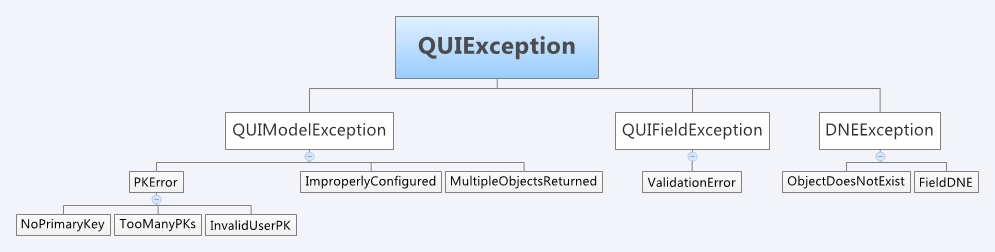
\includegraphics[width=450px]{ExceptionHierarchy}
\caption{QUI's exception hierarchy}
\label{fig:exceptionhier}
\end{figure}

Although these allow QUI to catch programmatic and procedural errors, we have not implemented an error handling system that intuits
probable \emph{desired} action; if commands are run which are `legal', according to QUI and Python syntax, no errors or warnings are raised---
no matter what the effect of those commands are.

\subsection{Tool Support}
As an internal DSL, QUI ``programs'' can be written in any environment in which Python programs can be written; the one is a subset of the 
other. There are no development environments that are \emph{specifically} designed to support or aid QUI programming, but most quality
development environments provide class introspection and code completion, which we have found more than sufficient for our own
purposes. 

Admittedly, we are more familiar with QUI than might be said is average, so your mileage may vary.

\subsection{Alternatives to QUI}
There are a few interfaces which share a common purpose with QUI -- the universalization of database access. None, however,
make it their focus to unify \emph{non-relational} databases. Packages like SQLAlchemy and Django's proprietary ORM work to
universalize access to many SQL-based relational databases, but neither officially supports non-relational databases of any sort.

QUI attempts to address an untapped niche market; its declared purpose is unique amongst ORMs.
\newpage
%%%%%%%%%%%%%%%%%%%%%%%%%%%%%%%%	SECTION 3	%%%%%%%%%%%%%%%%%%%%%%%%%%%%%%%%%%%
\section{Example Programs}
\label{examples}
\subsection{Model Definition}
Here's what it might look like if you wanted to define a simple model:
\lstdump[filemodel.py][defining a simple model]{model_definitions.py}

\il{FileModel}'s family tree, after decoration, looks like this:
\begin{figure}[htb]
\centering
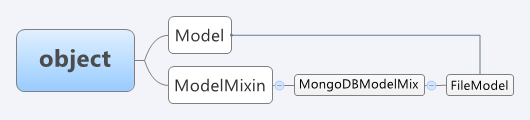
\includegraphics[width=400px]{FileModelInheritanceTree}
\caption{\il{FileModel}'s family tree.}
\end{figure}

\subsubsection{Step-by-step}
Let's step through this definition. First, we import the necesassary things from qui:
\lstslice{1}{4}{model_definitions.py}
\il{qui.fields} contains all the supported field types, like \il{StringField, IntegerField}, etc. At the moment, QUI supports 
a bare minimum of fields - just the most basic types.

Next, we decorate the class with \il{storage()}:

\lstslice{6}{7}{model_definitions.py}

the \il{backend} keyword argument to the \il{storage} decorator tells QUI which mixins it needs to add to your model's inheritance tree,
as well as the inheritance trees of any \il{Fields} you've defined for the model. \il{storage} will accept arbitrary keyword arguments,
but only acts on a few:
\begin{enumerate}
	\item \il{backend}, which defaults to \il{None} and will (generally) raise an \il{ImproperlyConfigured} exception if not defined, or
	if you pass in a backend-identifying string that isn't recognized.
	\item \il{host}, which takes a string and defaults to \il{'localhost'}.
	\item \il{db}, which takes a string and defaults to a backend-specific value.
	\item \il{port}, which takes an integer, and defaults to a backend-specific port.
\end{enumerate}
Our simple \il{FileModel}, then, uses the MongoDB backend, and will be stored locally, with default settings. Any subclasses of \il{FileModel}
will autoatically inherit these settings, but fine control is possible by defining \il{_host, _db, _port} on the subclass in question. If, for whatever
reason, we decided we'd rather store \il{FileModel}s using Pickling (for example), we'd have to change line 6 to \il{@stored(backend='Pickle')}, 
and QUI would acquiesce, no questions asked.

Next, we set some fields that we think a \il{FileModel} should have:
\lstslice{18}{27}{model_definitions.py}
Notice that we don't \emph{initialize} any of the fields here - we're just defining what kind of \il{Field} each attribute should be.
Although QUI will store any attributes that an instance of \il{FileModel} may have (except private ones and callable ones), these
\il{Field} attributes will do run-time compatibility checking. For example:

\lstsession[demonstrating run-time validation]{interpreter2.py}

\il{count} has been marked as a class attribute by the \il{class_field} decorator, and it will behave just like any other class attribute.
Also, notice that you can still have ``regular'' class variables, like \il{class_var}; these will be stored by QUI just like all other non-callable
attributes.

There's a (pedantic) function definition, just to show that we can, and (finally) we have \il{__unicode__}, which controls the way that a QUI model is printed via the \il{print} commands. :
\lstslice{29}{37}{model_definitions.py}
Since \il{my_size} is a callable, QUI ignores it - but doesn't remove it from the model. 
\lstsession[using fields with functions]{interpreter1.py}



\subsubsection{Subclassing a Model}
\lstdump[file\_subclasses.py][subclassing from FileModel]{subclassing.py}
This is just an example of a few ways that you can customize your QUI models. \il{ImageFile} is a direct subclass of \il{FileModel}, and has no further customizations.
QUI will store it instances of \il{ImageFile} in a different `place' than it does instances of \il{FileModel}, if that makes sense for the backend.

\il{TextFile} shows that you can define further \il{Field}s or regular class member variables, as you'd expect from a subclass.

\il{MoreClassFields} demonstrates the \il{subclass} decorator, which is only needed if your subclass defines more class-wide \il{Field}s. 

\il{Remote_File} exhibits the ability to redefine where the model should be stored, by customizing \il{_host} and \il{_port} members. The difference between defining them as class members and as instance members is subtle: all QUI functions will use the class member values, if they exist; only \il{put()} will use the instance values. So, \il{Remote_Files} will be \textbf{gotten} from the wherever \il{FileModel} has said to find them, but will be \textbf{put} to wherever \il{_host} has been initialized to. In this case, if \il{x = Remote_File.create('otherhost')}, it will be \il{create}d to \il{FileModel}'s host (localhost), but on port \il{91711}. Then \il{x.put()} will store it on otherhost, also using port \il{91711}. This feature is great for migrating data between hosts; you'll be \il{get()}ing from one host and \il{put()}ing to another!

Note that if you define a custom \il{__init__}, you also need to call \il{super}'s \il{__init__}  before you start modifying any instance attributes, so that QUI can do the necessary setup.

\subsubsection{Regarding Fields}
We really can't stress enough that you generally \emph{do not initialize \il{Field}s yourself}. All direct subclasses of \il{Field} are abstract, and even if they weren't, they do not define all the methods that \il{Field} requires in order to be instantiated. They have to be combined with a subclass of \il{FieldMixin} which fulfills their remaining requirements.

\begin{figure}[htb]
\centering
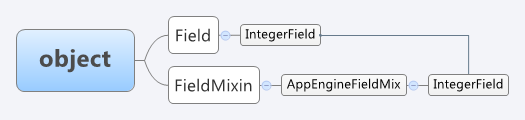
\includegraphics[width=400px]{IntegerFieldlInheritanceTreeforFileModel}
\caption{A family tree for \il{FileModel.size}.}
\end{figure}
 QUI does this for you when you decorate a class definition, and instantiates the resulting fields at the appropriate times---so that every \il{FileModel} has its own \il{name}, but the same \il{count}.
Defining \il{Field}s on your model isn't required; one of the best parts about non-relational databases is that they don't enforce a strict schema. Remember \il{x}, from above? If we had,
somewhere down the line, decided that \il{x.sensitive = True}, QUI would happily store the \il{sensitive} attribute right along with all of \il{x}'s other attributes. Defining an attribute as a
\il{Field} is mostly useful for enforcing a type, or coercing into a certain format:
\begin{inset}
\begin{lstlisting}
 >>> x.name = 123
 >>> x.name
 u'123'
\end{lstlisting}
\end{inset}

\subsection{Using QUI}
QUI's ease of use is best exhibited by entering the Python interpreter:

\lstsession[creating an instance with arbitrary attributes]{getting_and_setting.py}

This session doesn't show much that we haven't already seen; note that \il{f} has been created with an attribute that doesn't exist on the model's `hardcoded' definition,
and QUI is totally fine with it. Just as it works in the interpreter, so to will it work in any other Python-executing environment. 

\newpage
%%%%%%%%%%%%%%%%%%%%%%%%%%%%%%%%	SECTION 4	%%%%%%%%%%%%%%%%%%%%%%%%%%%%%%%%%%%
\section{Language Design}

\subsection{Getting, Putting, and Creating}
The idea behind QUI is to support a uniform set of `verbs' across all backends. As an internal language focusing on storage, we implemented
these verbs as class methods and instance methods.

Since our time for this project was limited, we focused our efforts on what we saw as the three most important verbs for a persistent storage solution:
\begin{enumerate}
\item \textbf{Creating} an instance of a stored model, at run-time, on the fly, and having it stored into the backend.
\item \textbf{Putting} an instance of a stored model into the backend.
\item \textbf{Getting} an instance of a stored model from the data stored in the backend.
\end{enumerate}
This tight focus on basic database operations also means there is almost no difficulty in learning QUI's syntax; the method of decorating a class as ``storable'' is also
incredibly simple, especially if the user is satsified to use QUI's default settings.

\subsection{Syntax}
As has been said repeatedly, QUI is an internal DSL; its syntax is no different from that allowed in any valid Python program. 
Nevertheless, QUI strives (in true Pythonic style) for an optimal combination of clarity and concision. It achieves this by only officially 
exposing three extra methods on stored models to users: \il{get(**kwargs)}, \il{create(**kwargs)}, and \il{put()}.

By only adding these three verbs to any \il{Model} definition, QUI runs the least risk of becoming a burden to anyone who decides to use
it; furthermore, these method names are unlikely to be already overridden. QUI doesn't want to step on anybody's toes, after all. 

Most of QUI's syntax is covered in Section~\ref{examples}; the example \il{Model} definitions and interpreter sessions cover the fundamentals,
and even some non-fundamentals, of using QUI pretty extensively. The user has a large amount of power when decided how exactly to create their
\il{Model}s, and are able to give the \il{Model} functionality in whatever manner they deem fit.

\subsection{Semantic Abstractions/Building Blocks}
QUI is abstracted into a number of different, though related sections. The user creates some sort of model (e.g., a \il{FileModel}), and performs \il{put, get,} and \il{create} operations as needed (they can also create other subclasses or functions within the \il{FileModel} class). At the top of the file (for now), users must import
our Model, any fields they want to use, and any decorators they want to use. 

Under the hood, operations become more complex for each API.  At its core, however, QUI uses the 'black box' of the API for each backend database, and accesses methods
as necessary to create, put, or get model instances. The user inputs commands using their created file (see examples above), which is decorated to use the appropriate backend mixins. 
These decorators call the appropriate \il{Field} and \il{Model} mixins so attributes are properly assigned and stored depending on the backend. The user should never see any actual 
database operations; QUI will handle all connections and operations necessary beyond the user's call to get, put, or create.

\newpage
%%%%%%%%%%%%%%%%%%%%%%%%%%%%%%%%	SECTION 5	%%%%%%%%%%%%%%%%%%%%%%%%%%%%%%%%%%%
\section{Language Implementation}
\subsection{Host Language}
QUI is implemented in Python, which was chosen for three main reasons:
\begin{enumerate}
\item Our own familiarity with the language.
\item Excellent metaprogramming facilities.
\item Availability of backend APIs.
\end{enumerate}
In a big way, our vision of QUI's design steered us towards Python as the host language. 

\subsection{Parsing}
As an internal DSL, it's unnecessary for QUI to perform any `parsing' operations, in the same sense as an external one --- there's no need for an abstract syntax tree, as QUI syntax
is merely Python syntax. In addition, we can rely on Python to catch syntactically illegal expressions in many cases. The most parsing that QUI ever does is on arguments to functions,
and these operate like flags or switches, determining flow through the various operations that QUI supports.

\subsection{Execution}
As an internal DSL, QUI's semantics do not differ from those of its host language, Python. Figure~\ref{fig:classdef} describes the operations that QUI is doing behind the scenes when
a class is decorated with \il{storage}.
\begin{figure}[htb]
\centering
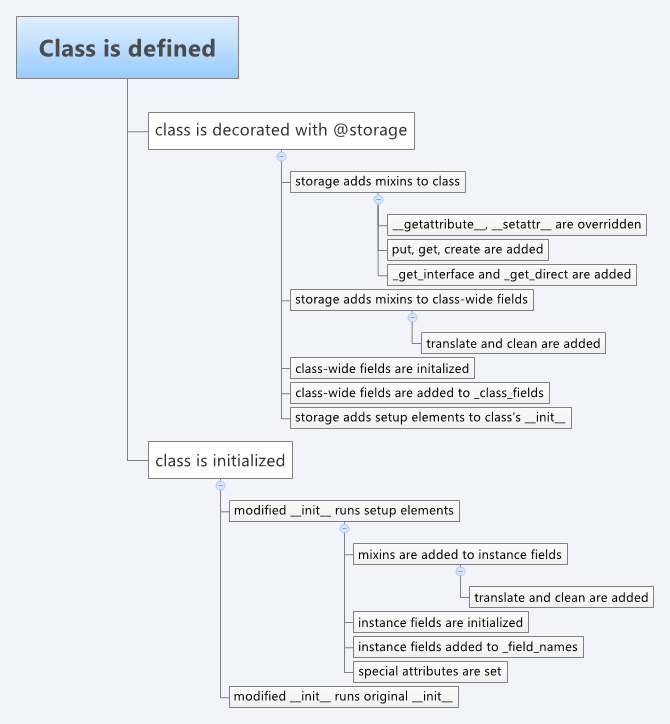
\includegraphics[width=400px]{ClassDefTimeline}
\caption{QUI's order of operations}
\label{fig:classdef}
\end{figure}
The \il{subclass} decorator is similar, but only performs the operations relating to class-wide fields, since a subclass of a QUI model will already have much of the setup done by its parent class. 

\subsection{Backends}
Currently, two backends are supported. 
\subsubsection{MongoDB}
	MongoDB is a  popular, free non-relational database. For putting, model instances are converted to JSON, and then saved in a database via some port. The port default is 27017,
	but the user can specify the port via passed in arguments. The \il{\_get\_interface()} method takes the model instance and sets each field as a key:value pair in the JSON
	dict.

	Getting is simply a matter of finding the object which corresponds to the passed in keyword arguments.
	
\subsubsection{Pickling}
	Also supported is local storage of model instances, using the Python pickle module. Model instances are stored in the directory specified by the \il{\_path} variable, in
	the file $Modelname\backslash InstancePrimaryKey$. Sadly, Python's pickle module will only pickle global classes (namely, not our \il{Model}s), so this backend simply pickles a dict
	which contains the state of the model instance.	
			
\newpage	
\section{Evaluation}
The basic implementation of QUI went as planned, building the framework for adding various backends. Adding a new backend is a nontrivial task, but only one file needs to be added
(\il{NewBackEndMixins.py}) defining the necessary classes, and QUI will take care of performing the operations for a \il{Model} decorated to use that backend (\il{@stored(backend='NewBackEnd')}).

Likewise, QUI's syntax is clear and concise, providing basic functionality while allowing the user full access to the power of Python. The user is free to use our built-in backend mixins, or 
to define their own if they so wish. This is well in keeping with the idea of non-relational databases: to give the user the flexibility they need to extend their applications in whatever
directions they wish to go. Furthermore, we built in several `escape hatches,' to allow users to avoid QUI's topmost layer, if desired: methods like \il{_get_direct()} allow a user to
directly access a \il{Field}, bypassing \il{Model}'s overridden \il{__getattribute__} and \il{__setattr__} entirely.

However, some difficulties were encountered in the implementation of QUI. Our initial intention was to use Google AppEngine as another backend, but upon investigation into the AppEngine
datastore, we found that AppEngine supports a non-relational database solely for applications on Google AppEngine. Pulling out just the datastore connection proved essentially impossible 
without a working application online. In light of this, providing support for just the AppEngine database seemed both overly time-consuming and unlikely to benefit any users, as they
still have to use other AppEngine functionalities to access their datastores. So, we focused on MongoDB and Pickling as our supported backends.

Time constraints also presented an issue during later development. The two methods required for specific backend FieldMixins have not yet been fully implemented, as 
they have almost no impact on the usability of the database and were added as a potential feature that might be convenient to users. The method \il{translate()} currently returns the 
value of a field, but would in the future convert a top-level \il{StringField()} (for example) to a \il{db.StringProperty()}, or whatever is appropriate for that backend. We also didn't have
time to override \emph{class} versions of \il{__getattribute__} and \il{__setattr__}, which involves some interesting work with metaclasses---so to access a class-wide \il{Field}'s value, 
you have to directly access its \il{value} attribute.

Likewise, the method \il{clean()} is intended to sanitize data before it is inserted into the database.

QUI was developed and implemented as a team. The initial design was done entirely on whiteboards with both participants working together.

  Later in the process, pair programming was used, with both members working on one computer. This was the abstract base classes and later the classes for the mixins to inherit. 
  
  The last stage of the project was actually developing for the backends. The backends were split between the two team members, though both had input in each backend --- for example, the
   decision to stop trying to support AppEngine as a backend was made as a team.

\newpage
\appendix
\begin{center}Appendices\end{center}

\section{Non-Relational Databases}
Non-relational databases differ distinctly from their more popular cousins. Relational databases adhere to the more traditional structure of some number of tables, linked
by specific keys, with some number of rows and columns. Every row in a specific table must have some specific attributes (the columns of the table), the same as every 
other row of the table. Adding a column to a table then requires stopping all interactions on that table, as every entry must be changed. 

Non-relational databases are not as restricted in their structure (see Figure~\ref{fig:reltab}). Rather than each entry being a row in a table with a fixed number of 
columns, each model instance is a 'page' in the database, with its own fields (some of which may be required, and others specific to the instance itself). So, 
non-relational databases are much more horizontally flexible when freezing the database would be inopportune if a new field needs to be added.

Implementations of non-relational databases vary widely between backends, but the main idea of non-relational databases is removing the field restriction for the user.
One of QUI's basic goals is to preserve this functionality. 
\begin{figure}[htb]
\centering
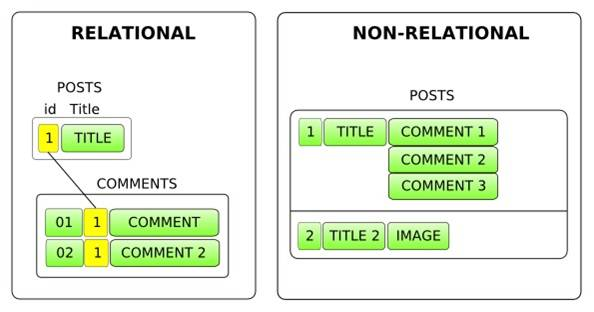
\includegraphics[width=300px]{RelNonRel}
\caption{Relational vs. Non-Relational (source: readwriteweb.com) }
\label{fig:reltab}
\end{figure}


\end{document}
